% ------------------------------------------------------------------------------ %

  \documentclass[a4paper,11pt]{report}

% ------------------------------------------------------------------------------- %
%LANGUAGE PACKS%

  \usepackage[english]{babel} 
 % ------------------------------------------------------------------------------- %
%FONTS%    
  \usepackage[utf8x]{inputenc}
  
  \usepackage{amsmath}
  \usepackage{multirow}
  \usepackage{enumerate}
  \usepackage{verbatim}
  \usepackage{listings}
% ------------------------------------------------------------------------------- %
%LAYOUT%  

\usepackage{fullpage}

 \tolerance=1
 \emergencystretch=\maxdimen
 \hyphenpenalty=10000
 \hbadness=10000
 \newcommand{\HRule}{\rule{\linewidth}{0.5mm}}
 
 \usepackage[pdftex]{graphicx} 

 
 \usepackage{hyperref}

 \hypersetup{
    colorlinks,
    citecolor=black,
    filecolor=black,
    linkcolor=black,
    urlcolor=black
}
\lstset {breaklines=true,
extendedchars=false,
showstringspaces=false}

% ------------------------------------------------------------------------------- %

% ------------------------------------------------------------------------------- %


\begin{document}

\begin{titlepage}

\begin{center}


\includegraphics{images/UvA-logo-2a.png}~\\[1cm]

\textsc{\LARGE System and Network Engineering, OS3 Group}\\[1.5cm]

\HRule \\

{ \huge \bfseries Essential Skills\\Latex Assignment}

\HRule \\[1cm]

\large{Diana Rusu} \\
\large{Alex Stavroulakis}\\
\large{Nick Triantafylldis}\\


\end{center}
\end{titlepage}

\tableofcontents

\chapter* {Introduction}
\addcontentsline{toc}{chapter}{Introduction}

This is our report in latex.

\chapter{XML in the Semantic web : RDF}


\section{Semantic Web}

\paragraph{}Semantic Web is a framework for sharing data between applications, enterprises and people, independent of platform and software(W3C).

Semantic refers to meaning. It is "a web of data that can be processed directly and indirectly by machines" - Tim Berners Lee

Extends the internet which comprises web-pages readable only to humans, to websites that use metadata and can be read by machines.

This leads to the creation of "smart" services that can perform tasks for users with better results and help them share and fin info more easier.

Example : A human can utilize the web to search, find, compare and choose the lowest price to a product. Machines cannot since the webpages aren't build to be read b them.

Semantic Web is a form of information that can be interpreted by machines so they can accomplish the tedious tasks that contain searching, putting together and editing what's already available online.
\paragraph{}

\begin{center}
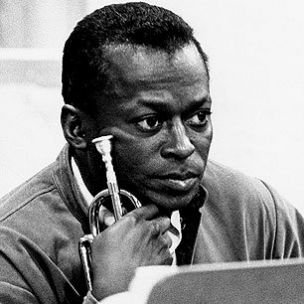
\includegraphics[width=90mm]{images/semantic-web-3.jpg}~\\[1cm]
A URI gives a computer a specific point of reference for each item in the triple -- there is no need or interpretation or potential for misunderstanding.

\url {http://computer.howstuffworks.com/semantic-web3.htm
} 
\end{center}

\section{RDF}
\paragraph{}
RDF short for Resource Description Framework language is a cross-platform framework for describing resources on the web.

XML-based RDF allows a common way to describe and share information between different types of applications operating systems and computers.


Slide presentation for this topic can be found on the following link : \url{https://docs.google.com/file/d/0BzZaPwl3dLnFeW0tZGV5bHdRNUU/edit?usp=docslist_api}


\subsection{RDF Example}

 
Here are two records from a CD-list:
 
\begin{center} 
\begin{tabular}{ | l | c | c | c | c | c |}
 \hline
 Title & Artist & Country & Company & Price & Year \\ \hline
 Empire Burlesque & Bob Dylan & USA &	Columbia & 10.90 &	1985 \\
 \hline
  Hide your heart & Bonnie Tyler & UK &	CBS Records &9.90 &	1988 \\
 \hline
\end{tabular}
\end{center}
Source : \url{http://www.w3schools.com/webservices/ws_rdf_example.asp}
\paragraph{}
Below is a few lines from an RDF document:

\begin{lstlisting}[language=XML]
<?xml version="1.0"?>
<rdf:RDF
xmlns:rdf="http://www.w3.org/1999/02/22-rdf-syntax-ns#"
xmlns:cd="http://www.recshop.fake/cd#">

<rdf:Description
rdf:about="http://www.recshop.fake/cd/Empire Burlesque">
  <cd:artist>Bob Dylan</cd:artist>
  <cd:country>USA</cd:country>
  <cd:company>Columbia</cd:company>
  <cd:price>10.90</cd:price>
  <cd:year>1985</cd:year>
</rdf:Description>

<rdf:Description
rdf:about="http://www.recshop.fake/cd/Hide your heart">
  <cd:artist>Bonnie Tyler</cd:artist>
  <cd:country>UK</cd:country>
  <cd:company>CBS Records</cd:company>
  <cd:price>9.90</cd:price>
  <cd:year>1988</cd:year>
</rdf:Description>
.
.
.
</rdf:RDF> 


\end{lstlisting}
\paragraph{}
The first line of the RDF document is the XML declaration. The XML declaration is followed by the root element of RDF documents: \textbf{\textless rdf:RDF\textgreater}.

The xmlns:rdf namespace, specifies that elements with the rdf prefix are from the namespace "http://www.w3.org/1999/02/22-rdf-syntax-ns\#".

The xmlns:cd namespace, specifies that elements with the cd prefix are from the namespace "http://www.recshop.fake/cd\#".

The \textless rdf:Description\textgreater element contains the description of the resource identified by the rdf:about attribute.

The elements: \textbf{\textless cd:artist\textgreater}, \textbf{\textless cd:country\textgreater}, \textbf{\textless cd:company}\textgreater, etc. are properties of the resource.

\end{document}





